\documentclass[a4paper,12pt]{article}
\usepackage[utf8]{inputenc}
\usepackage{tikz}
\usetikzlibrary{arrows.meta, positioning}

\title{TikZ: Eksempler på \texttt{\textbackslash draw}}
\author{}
\date{}

\begin{document}
\maketitle

\section*{Grunnleggende linje}
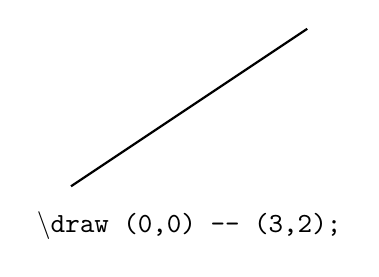
\begin{tikzpicture}
  \draw[thick] (0,0) -- (3,2);
  \node at (1.5,-0.5) {\texttt{\textbackslash draw (0,0) -- (3,2);}};
\end{tikzpicture}

\vspace{1cm}

\section*{Rektangel og fyllfarge}
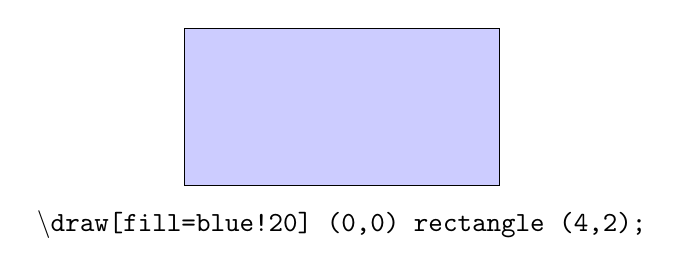
\begin{tikzpicture}
  \draw[fill=blue!20] (0,0) rectangle (4,2);
  \node at (2,-0.5) {\texttt{\textbackslash draw[fill=blue!20] (0,0) rectangle (4,2);}};
\end{tikzpicture}

\vspace{1cm}

\section*{Lukket figur med \texttt{cycle}}
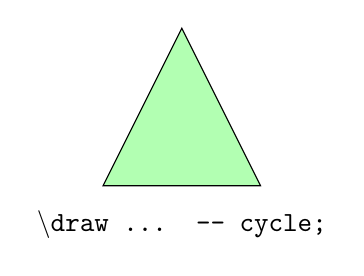
\begin{tikzpicture}
  \draw[fill=green!30] (0,0) -- (2,0) -- (1,2) -- cycle;
  \node at (1,-0.5) {\texttt{\textbackslash draw ... -- cycle;}};
\end{tikzpicture}

\vspace{1cm}

\section*{Linjestiler}
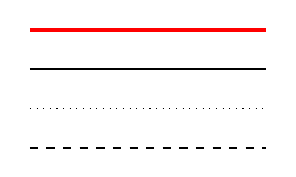
\begin{tikzpicture}
  \draw[dashed] (0,0) -- (3,0);
  \draw[dotted] (0,0.5) -- (3,0.5);
  \draw[thick] (0,1) -- (3,1);
  \draw[ultra thick, red] (0,1.5) -- (3,1.5);
\end{tikzpicture}

\vspace{1cm}

\section*{Piler}
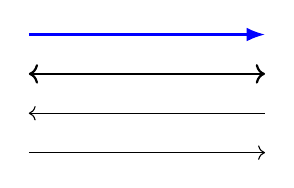
\begin{tikzpicture}
  \draw[->] (0,0) -- (3,0);
  \draw[<-] (0,0.5) -- (3,0.5);
  \draw[<->, thick] (0,1) -- (3,1);
  \draw[-{Latex}, blue, thick] (0,1.5) -- (3,1.5);
\end{tikzpicture}

\vspace{1cm}

\section*{Kurver med kontrollpunkter}
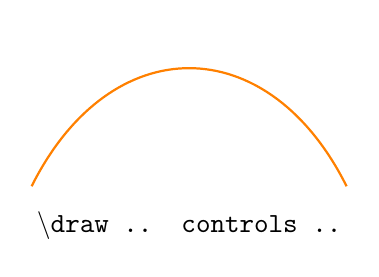
\begin{tikzpicture}
  \draw[thick, orange] (0,0) .. controls (1,2) and (3,2) .. (4,0);
  \node at (2,-0.5) {\texttt{\textbackslash draw .. controls ..}};
\end{tikzpicture}

\vspace{1cm}

\section*{Rutenett og akser}
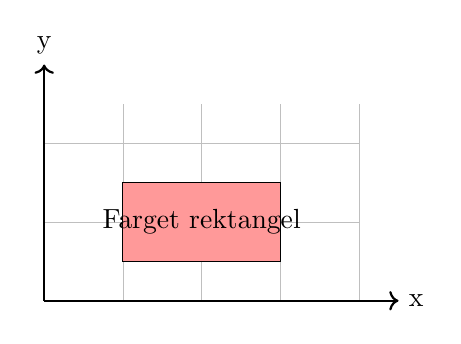
\begin{tikzpicture}[x=0.5cm, y=0.5cm]
  \draw[step=1cm, gray!50, very thin] (0,0) grid (8,5);
  \draw[->, thick] (0,0) -- (9,0) node[right] {x};
  \draw[->, thick] (0,0) -- (0,6) node[above] {y};
  \draw[fill=red!40] (2,1) rectangle (6,3);
  \node at (4,2) {Farget rektangel};
\end{tikzpicture}

\vspace{1cm}

\section*{Noder og merknader}
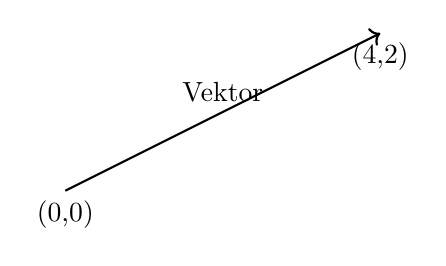
\begin{tikzpicture}
  \draw[->, thick] (0,0) -- (4,2) node[midway, above] {Vektor};
  \node[below] at (0,0) {(0,0)};
  \node[below] at (4,2) {(4,2)};
\end{tikzpicture}

\vspace{1cm}

\section*{Rundede hjørner}
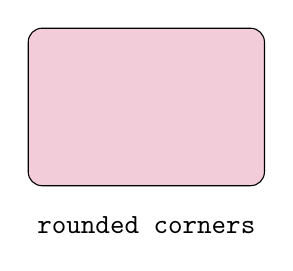
\begin{tikzpicture}
  \draw[fill=purple!20, rounded corners=5pt] (0,0) -- (3,0) -- (3,2) -- (0,2) -- cycle;
  \node at (1.5,-0.5) {\texttt{rounded corners}};
\end{tikzpicture}

\vspace{1cm}
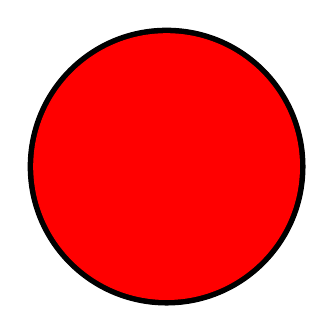
\begin{tikzpicture}
    \filldraw [black] (0,0) circle (50pt);    
    \filldraw [red] (0,0) circle (48pt);    
\end{tikzpicture}
         

\end{document}